\documentclass[a4paper, 10pt]{article}
%\usepackage[utf8]{inputenc}			
\usepackage[english]{babel}		% for german	
\usepackage[dvips]{graphicx}		
\usepackage{graphicx}	
\usepackage{psfrag}						
\usepackage{parskip}
\usepackage{listings}
\usepackage{xcolor}
\usepackage{amsmath}
\usepackage{mathtools}
\usepackage{amssymb}
\usepackage{mathrsfs}
\usepackage{empheq}
\usepackage{titlesec}	
\usepackage{pdfpages}
\usepackage{tikz}
\usetikzlibrary{arrows, shapes}
\usepackage{epstopdf}
\usepackage{dsfont}
\usepackage{sectsty}
\allsectionsfont{\bfseries\sffamily}

\addtolength{\textwidth}{2.1cm}
\addtolength{\topmargin}{-1.4cm}
\addtolength{\oddsidemargin}{-1.1 cm}
\definecolor{leichtgrau}{gray}{0.91}
\setlength{\parindent}{0pt}

% \lstset{language = C,
	% basicstyle=\footnotesize,       
	% numbers=left,                  
	% numberstyle=\footnotesize,      
	% stepnumber=2,
	% numbersep=5pt,
	% backgroundcolor=\color{leichtgrau},
	% frame=single,
% }

% Definition von römischen Zahlen
\makeatletter
\newcommand{\rmnum}[1]{\romannumeral #1}
\newcommand{\Rmnum}[1]{\expandafter\@slowromancap\romannumeral #1@}
\makeatother
%\renewcommand{\familydefault}{\sfdefault}
\title{MIMO Skript\,-\,Wintersemester 2013 \\ Kapitel 4}
\date{}

\begin{document}

\maketitle
\tableofcontents
\setcounter{section}{3}
\section{Distributed MIMO}

\begin{itemize}
	\item This research topic emerged ca. 10 years ago and is still a very active area of research
	\item Simple relaying schemes have been included in recent standards such as IEEE 802.16 (WiMAX) and LTE\,-\,Advanced
	\item Advantages: relay\,-\,assisted communications:
	\begin{itemize}
		\item Relays can help to reduce the effective overall pathloss
		\item Relays can also combat small\,-\,scale fading effects
		\item Relays can help to realize MIMO gains with single\,-\,antenna nodes
	\end{itemize}
	\item Challenges in relays\,-\,assisted communication:
	\begin{itemize}
		\item Network architectures are becoming more complex
		\item Synchronization across different nodes may be necessary \textit{(Anm.: untersch. Tr\"agerfrequenzen der Relays $\rightarrow $ Offset, Fehler, etc.)}
		\item Exchange of channel state information (CSI) across nodes may be required
	\end{itemize}
\end{itemize}

\subsection{Half\,-\,Duplex One\,-\,Way Relaying}
\paragraph{Basic Relay Network}
\begin{figure}[ht]
	\centering
	\psfrag{h_SR}[bl][bl][1]{$h_{SR}$}
	\psfrag{h_RD}[bl][bl][1]{$h_{RD}$}
	\psfrag{h_SD}[bl][bl][1]{$h_{SD}$}
	\includegraphics[scale=2]{Basic_Relay_Network}	
	\caption{Basic Relay Network}
	\label{fig:basic_relay_network}
\end{figure}
\begin{itemize}
	\item Relay R assists source S in communication with destination D
	\item Two basic nodes of transmission (at the relay):
\end{itemize}
\paragraph{Full\,-\,Duplex relaying:} 
R can receive and transmit at the same time and in the same frequency band \textit{(Anm.: effizient, da restliche Zeit und restliche Frequenzband von anderen genutzt werden kann)}
\begin{itemize}
	\item[$\rightarrow$] Since the TX signal power is orders of magnitude larger than the RX power, there is self\,-\,interference (at the relay) 
		\begin{figure}[ht]
			\centering
			\psfrag{y_R}[bl][bl][1]{$y_{R}$}
			\psfrag{s_R}[bl][bl][1]{$s_{R}$}
			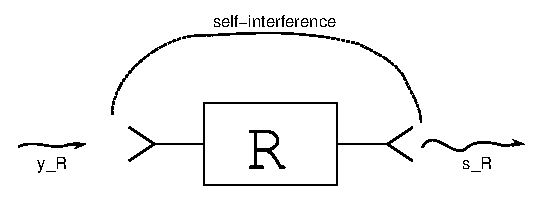
\includegraphics[scale=1]{Relay_self_interference}	
			\caption{Relay with self-interference}
			\label{fig:relay_self_interference}
		\end{figure}	
	\item[$\rightarrow$] Full\,-\,duplex relays are difficult to implement. The design of full\,-\,duplex relays is an active area of research.
	\item[$\rightarrow$] Majority of existing literature assumes half\,-\,duplex relaying.
\end{itemize}
\paragraph{Half\,-\,duplex relaying:} 
R transmits and receives in different time slots and/\,or different frequency bands. Typically, a two\,-\,phase protocoll is used:
\begin{itemize}
	\item[] \textbf{Phase 1}: S transmits, R and D receive 
	\begin{figure}[ht]
		\centering
		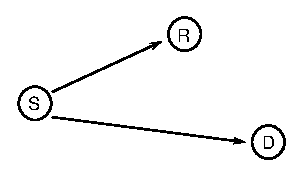
\includegraphics[scale=1.3]{Relay_HalfDuplex_1}	
		\caption{Half-duplex Relaying: Phase 1}
		\label{fig:relay_halfduplex_1}
	\end{figure}
	\item[] \textbf{Phase 2}: R transmits, D receives, S may or may not transmit 
	\begin{figure}[ht]
		\centering
		\includegraphics[scale=1.3]{Relay_HalfDuplex_2}	
		\caption{Half-duplex Relaying: Phase 2}
		\label{fig:relay_halfduplex_2}
	\end{figure}
\end{itemize}
There are different relaying strategies that differ in the processing applied at the relay. The most popular are:
\begin{itemize}
	\item Decode\,-\,and\,-\,Forward
	\item Amplify\,-\,and\,-\,Forward
	\item (Compress\,-\,and\,-\,Forward)
\end{itemize}

\subsubsection{Decode\,-\,and\,-\,Forward (DF) Relaying}
In DF relaying, the relay detects and decodes the signal received from the source before encoding it and  forwarding it to the destination.
	\begin{figure}[ht]
		\centering
		\psfrag{h_SR}[bl][bl][1]{$h_{SR}$}
		\psfrag{h_RD}[bl][bl][1]{$h_{RD}$}
		\psfrag{h_SD}[bl][bl][1]{$h_{SD}$}
		\psfrag{y_R}[bl][bl][1]{$y_R$}
		\psfrag{y_D1}[bl][bl][1]{$y_{D,1}$}
		\psfrag{y_D2}[bl][bl][1]{$y_{D,2}$}
		\psfrag{x_R}[bl][bl][1]{$x_R$}		
		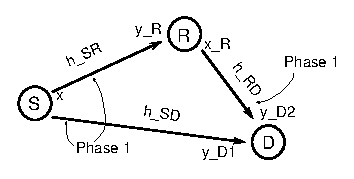
\includegraphics[scale=1.5]{DF_Relaying}	
		\caption{Block diagramm Decode\,-\,and\,-\,forward Relaying}
		\label{fig:df_relaying}
	\end{figure}
\paragraph{Phase 1:}
\begin{itemize}
	\item R receives: $ y_R = h_{SR}x + n_R $
	\item D receives: $ y_{D1} = h_{SD}x + n_{D1} $
	\item with: 
	\begin{itemize}
		\item transmit signal $x, \mathcal{E}_s = \mathcal{E}\{|x|^2\} $
		\item AWGN $n_R $ and $ n_{D1}$, $\sigma_n^2 = \mathcal{E}\{|n_R|^2\} = \mathcal{E}\{|n_{D1}|^2\} $
	\end{itemize}
\end{itemize}
\paragraph{Phase 2:}
\begin{itemize}
	\item R decodes and forwards $x_R$ (estimate of $x$)
	\item D receives: $ y_{D2} = h_{RD}x_R + n_{D2} $
	\begin{itemize}
		\item $x_R$ is estimate of $x $ after decoding at R
		\item $\sigma_n^2 = \mathcal{E}\{|n_{D2}|^2\}\,;\quad \mathcal{E}_R = \mathcal{E}\{|x_R|^2\} $
		\item weassume: S is silent in Phase 2		 
	\end{itemize}
\end{itemize}
\paragraph{}
\begin{itemize}
	\item The capacity at the three node relay channel is not known!
	\item We provide an achievable rate under the following simplifying assumption: The direct source\,-\,relay link is not used/\,exploited.
	\item Achievable rate without S\,-\,D link:
	\begin{align*}
		\boxed{C_{DF} = \frac{1}{2}\text{min}\bigl\{\log_2\bigl(1 + \frac{\mathcal{E}_S|h_{SR}|^2}{\sigma_n^2}\bigr),\,\log_2\bigl(1 + \frac{\mathcal{E}_R|h_{RD}|^2}{\sigma_n^2}\bigr)\bigr\} }	
	\end{align*}	 
	\begin{itemize}
		\item factor $\frac{1}{2} $ is due to the fact that we use two time slots to transmit one packet
		\item $\text{min}\{\ldots\} $ means we are limited by the weaker link (bottle\,-\,neck)
		\item If power allocation is possible, the total power $ \mathcal{E} = \mathcal{E}_S + \mathcal{E}_R $ should be divided between S and R to guarantee:
		\begin{align*}
			&\frac{\mathcal{E}_S|h_{SR}|^2}{\sigma_n^2} = \frac{\mathcal{E}_R|h_{RD}|^2}{\sigma_n^2},\\
			&\mathcal{E}_R = \frac{|h_{SR}|^2}{|h_{SR}|^2 + |h_{RD}|^2}\cdot\mathcal{E},\\
			&\mathcal{E}_S = \frac{|h_{RD}|^2}{|h_{SR}|^2 + |h_{RD}|^2}\cdot\mathcal{E}
		\end{align*}
	\end{itemize}
	\item Outage\,-\,probability in fading:
	\begin{itemize}
		\item We transmit with fixed rate R
		\item An outage occurs, if:
		\begin{align*}
			\frac{1}{2}\log_2\Bigl(1 + \underbrace{\frac{\mathcal{E}_S|h_{SR}|^2}{\sigma_n^2}}_{= \gamma_{SR}}\Bigr) &< R \quad	\text{or} \\
			\frac{1}{2}\log_2\Bigl(1 + \underbrace{\frac{\mathcal{E}_R|h_{RD}|^2}{\sigma_n^2}}_{= \gamma_{RD}}\Bigr) &< R
		\end{align*}
		\begin{align*}
			\boxed{\gamma_{SR} < \underbrace{2^{2R} - 1}_{\gamma_T} \quad \text{or}\quad \gamma_{RD} < 2^{2R} - 1}
		\end{align*}
		\begin{align*}
			P_{\text{out}} &= \text{Pr}\bigl\{\gamma_{SR} < \gamma_T \vee \gamma_{RD} < \gamma_T\bigr\}
			= \text{Pr}\bigl\{\underbrace{\text{min}\bigl\{\gamma_{SR},\gamma_{RD}\bigr\}}_{ = \gamma_{eq}} < \gamma_T\bigr\} \\ &= 1- \text{Pr}\bigl\{\gamma_{SR} > \gamma_T \wedge \gamma_{RD} > \gamma_T\bigr\} = 1 - \text{Pr}\bigl\{\gamma_{SR} > \gamma_T\bigr\}\,\text{Pr}\bigl\{\gamma_{RD} > \gamma_T\bigr\} = \\ &= 1 - \bigl(1 - F_{\gamma_{SR}}(\gamma_T)\bigr)\bigl(1 - F_{\gamma_{RD}}(\gamma_T)\bigr) = \\ &= \underline{F_{\gamma_{SR}}(\gamma_T) + F_{\gamma_{RD}}(\gamma_T) - F_{\gamma_{SR}}(\gamma_T)\cdot F_{\gamma_{RD}}(\gamma_T)}
		\end{align*}
		\item[] with CDFs: $F_{\gamma_{SR}}(\cdot) $ and $F_{\gamma_{RD}}(\cdot) $ 
		\item Rayleigh Fading: 
		\begin{align*}
		\rightarrow	F_{\gamma_{SR}}(\gamma) &= 1-\exp\bigl(\frac{-\gamma}{\bar{\gamma}_{SR}}\bigr)\,;\quad \bar{\gamma}_{SR} = \mathcal{E}\{\gamma_{SR}\} \\
			F_{\gamma_{RD}}(\gamma) &= 1-\exp\bigl(\frac{-\gamma}{\bar{\gamma}_{RD}}\bigr)\,;\quad \bar{\gamma}_{RD} = \mathcal{E}\{\gamma_{RD}\}\\
		\rightarrow P_{\text{out}} &= 1-\exp\bigl(\frac{-\gamma_T}{\bar{\gamma}_{SR}}\bigr) + 1-\exp\bigl(\frac{-\gamma_T}{\bar{\gamma}_{RD}}\bigr) - \Bigl(1-\exp\bigl(\frac{-\gamma_T}{\bar{\gamma}_{SR}}\bigr)\Bigr)\Bigl( 1-\exp\bigl(\frac{-\gamma_T}{\bar{\gamma}_{RD}}\bigr)\Bigr) = \\
		&= 1 - \exp\Bigl(-\frac{\bar{\gamma}_{SR} + \bar{\gamma}_{RD}}{\bar{\gamma}_{SR}\bar{\gamma}_{RD}}	\cdot\gamma_T\Bigr)
		\end{align*}
		\item[$\rightarrow$] equivalent SNR $\gamma_{eq} = \min\bigl\{\gamma_{SR}, \gamma_{RD}\bigr\} $ is also exponentially distributed with \\ $\bar{\gamma}_{eq} = \frac{\bar{\gamma}_{SR}\bar{\gamma}_{RD}}{\bar{\gamma}_{SR} + \bar{\gamma}_{RD}} $ 
		\item Diversity gain: Assume $\bar{\gamma}_{SR} = \alpha\bar{\gamma} $
		\begin{align*}
			\rightarrow P_{out} & \xrightarrow{\bar{\gamma} \rightarrow \inf} 1 - \Bigl(1-\frac{\alpha + \beta}{\alpha\beta}\cdot\frac{\gamma_T}{\bar{\gamma}}\Bigr) + \mathcal{O}\bigl(\bar{\gamma}^{-1}\bigr) = \\ 
			&= \frac{\alpha + \beta}{\alpha\beta}\cdot\frac{\gamma_T}{\bar{\gamma}} + \mathcal{O}\bigl(\bar{\gamma}^{-1}\bigr) = \\
			& \rightarrow \boxed{G_d = 1}
		\end{align*}
	\end{itemize}
	\item Bit error rate (BER) of BPSK (uncoded)
	\begin{itemize}
		\item $\text{BER}\bigl(\gamma_{SR},\gamma_{RD}\bigr) = \Bigl(1 - \text{BER}_{SR}\bigl(\gamma_{SR}\bigl)\Bigl)\text{BER}_{RD}\bigl(\gamma_{RD}\bigr) + \Bigl(1 - \text{BER}_{RD}\bigl(\gamma_{RD}\bigl)\Bigl)\text{BER}_{SR}\bigl(\gamma_{SR}\bigr) $ 
		\begin{itemize}
			\item with BER of the S\,-\,R link, $\text{BER}_{SR}(\gamma_{SR}) $ and BER of the R\,-\,D link $\text{BER}_{RD}(\gamma_{RD}) $ 
			\item for sufficiently high SNR $\leadsto \text{BER}_{SR}(\gamma_{SR}), \text{BER}_{RD}(\gamma_{RD}) \ll \text{BER}_{SR}(\gamma_{SR}) + \text{BER}_{RD}(\gamma_{RD}) $
			\item[$\rightarrow$] $\underline{\text{BER}(\gamma_{SR},\gamma_{RD}) \approx \text{BER}_{SR}(\gamma_{SR}) + \text{BER}_{RD}(\gamma_{RD})} $
			\item to average BER (Rayleigh Fading):
			\begin{align*}
				\text{BER} = \mathcal{E}_{\gamma_{SR},\gamma_{RD}}\Bigl\{\text{BER}\bigl(\gamma_{SR},\gamma_{RD}\bigr)\Bigr\} = \frac{1}{2}\Bigl(1-\sqrt{\frac{1}{1+\frac{1}{\bar{\gamma}_{SR}}}} + \frac{1}{2}\Bigl(1-\sqrt{\frac{1}{1+\frac{1}{\bar{\gamma}_{RD}}}}\Bigr)
			\end{align*}
			\item high SNR: 
			\begin{align*}
				\text{BER} &\approx \frac{1}{2}\bigl(1 - 1 + \frac{1}{2}\frac{1}{\bar{\gamma}_{SR}}\bigr) + \frac{1}{2}\bigl(1 - 1 + \frac{1}{2}\frac{1}{\bar{\gamma}_{RD}}\bigr) = \\ 
				&= \frac{1}{4}\bigl(\frac{1}{\bar{\gamma}_{SR}} + \frac{1}{\bar{\gamma}_{RD}}\bigr)
			\end{align*}
			$\leadsto $ also indicates diversity gain $ G_d = 1 $
		\end{itemize}		 
	\end{itemize}
\end{itemize}
\subsubsection{Amplify\,-\,and\,-\,Forward (AF) Relaying}
\begin{itemize}
	\item Relay does not decode signal received from source but only amplifies it before forwarding it to the destination
	\begin{figure}[ht]
		\centering
		\psfrag{y_R}[bl][bl]{$y_R$}
		\psfrag{Ay_R}[bl][bl]{$Ay_R$}
		\psfrag{h_SR}[bl][bl]{$h_{SR}$}
		\psfrag{h_SD}[bl][bl]{$h_{SD}$}
		\psfrag{h_RD}[bl][bl]{$h_{RD}$}	
		\psfrag{y_D2}[bl][bl]{$y_{D,2}$}
		\psfrag{y_D1}[bl][bl]{$y_{D,1}$}
		\includegraphics[scale=1.5]{AF_Relaying}
		\caption{Block diagramm AF\,-\,Relaying}	
		\label{fig:af_relaying}
	\end{figure}
	\item Amplification gain $A $ may be constant on channel dependent and ensures a certain (average) transmit power
	\item[] \textbf{Phase 1}:
	\begin{itemize}
		\item[-] R receives: $y_D = h_{SR}x + n_R $
		\item[-] D receives: $y_{D,1} = h_{SD}x + n_{D,1} $
	\end{itemize}
	\item[] \textbf{Phase 2}:
	\begin{itemize}
		\item[-] R transmits: $s_R = Ay_R = A(h_{SR}x + n_R) $
		\item[-] D receives: $y_{D,2} = h_{RD}Ay_R + n_{D,2} $  
	\end{itemize}
	\item We can use MRC to combine $y_{D,1} $ and $ y_{D,2} $ at D: $ y_{D,2} = Ah_{RD}h_{SR}x + h_{RD}An_R + n_{D,2} $,\quad where: $ h_{RD}An_R + n_{D,2} $ is effective noise $n_{\text{eff}} $ with variance $\sigma_{n_\text{eff}}^2 = \sigma_n^2\bigl(|h_{RD}|^2A^2 + 1\bigr) $
	\item[$\rightarrow$] make noise variances of both branches equal
	\begin{align*}
		\bar{y}_{D,2} &= \frac{1}{\sqrt{|h_{RD}|^2A^2+1}}\cdot y_{D,2} = \frac{Ah_{RD}h_{SR}}{\sqrt{A^2|h_{RD}|^2 + 1}} \cdot x + \tilde{n}_{\text{eff}} \\
		\text{MRC:}\quad r &= h_{SD}^*y_{D,1} + \frac{Ah_{RD}^*h_{SR}^*}{\sqrt{A^2|h_{RD}|^2+1}}\cdot\bar{y}_{D,2} = \underbrace{h_{SD}^*y_{D,1} + \frac{Ah_{RD}^*h_{SR}^*}{A^2|h_{RD}|^2 + 1}\cdot y_{D,2}}_{ = \text{decision variable!}}		
	\end{align*}
	\item Choice of A: The goal is to ensure en (average) transmit power of $\mathcal{E}_R $	
\end{itemize}
\paragraph{a) Variable gain relaying:}
In this case we introduce an instantaneous power constraint. \textit{Anm.: A muss abh\"angig von $h_{SR} $ sein, um es kompensieren zu k\"onnen.}
\begin{align*}
	\mathcal{E}_{x,n}\bigl\{|S_R|^2\bigr\} &= \mathcal{E}_{x,n}\bigl\{A^2\bigl(|h_{SR}|^2|x|^2 + |n_R|^2\bigr)\bigr\} = \\ &= A^2\bigl(|h_{SR}|^2\mathcal{E}_S + \sigma_n^2\bigr) \overset{!}{=} \mathcal{E}_R \\ \rightarrow A^2 &= \frac{\mathcal{E}_R}{|h_{SR}|^2\mathcal{E}_S + \sigma_n^2}	 
\end{align*}
\begin{itemize}
	\item A is channel dependent
	\item Instantaneous transmit power is \underline{not} channel dependent 
\end{itemize}
\paragraph{b) Fixed gain relaying:} In this case, we introduce an average (with respect to the channel) power constraint
\begin{align*}
	\mathcal{E}\bigl\{|S_R|^2\bigr\} &= \mathcal{E}\bigl\{A^2\bigl(|h_{SR}|^2|x|^2 + |n_R|^2\bigr)\bigr\} = \\ &= A^2\bigl( \underbrace{\mathcal{E}\bigl\{|h_{SR}|^2\bigr\}}_{\sigma_{SR}^2}\mathcal{E}_S + \sigma_n^2\bigr) \overset{!}{=} \mathcal{E}_R \\ \rightarrow A^2 &= \frac{\mathcal{E}_R}{\mathcal{E}_S\sigma_{SR}^2 + \sigma_n^2}	 
\end{align*}
\begin{itemize}
	\item A is not channel dependent
	\item Instantaneous power of $S_R $ depends on channel and may actually vary widely
\end{itemize}
Equivalent SNR for variable gain AF relaying (inly relayed link)
\begin{align*}
	y_{D,2} = Ah_{RD}h_{SR}x + h_{RD}An_R + n_{D,2}
\end{align*}
\begin{align*}
	\text{SNR: }\quad \gamma_{eq}^{AF} &= \frac{A^2|h_{SR}|^2|h_{RD}|^2\mathcal{E}_S}{A^2|h_{RD}|^2\sigma_n^2 + \sigma_n^2} = \frac{\frac{\mathcal{E}_S}{\sigma_n^2}|h_{SR}|^2|h_{RD}|^2}{|h_{RD}|^2 + \frac{1}{\mathcal{E}_R}(|h_{SR}|^2\mathcal{E}_S + \sigma_n^2)} = \\ &= \frac{\frac{\mathcal{E}_S}{\sigma_n^2}|h_{SR}|^2\cdot\frac{\mathcal{E}_R}{\sigma_n^2}|h_{RD}|^2}{\frac{\mathcal{E}_R}{\sigma_n^2}|h_{RD}|^2 + \frac{\mathcal{E}_S}{\sigma_n^2}|h_{SR}|^2 + 1} = \\ &= \frac{\gamma_{SR}\gamma_{RD}}{\gamma_{SR} + \gamma_{RD} + 1}
\end{align*}
high SNR: $\gamma_{SR},\,\gamma_{RD} \gg 1 $
\begin{align}
	\boxed{\gamma_{eq}^{AF} = \frac{\gamma_{SR}\gamma_{RD}}{\gamma_{SR} + \gamma_{RD}}} \label{eq:Formel_01}
\end{align}
\textit{Anm.: Vgl. Formel \ref{eq:Formel_01} mit Berechnung zweier paralleler Widerst\"ande.}
Comparison with equivalent SNF of DF:
\begin{align}
	\boxed{\gamma_{eq}^{DF} = \min\bigl\{\gamma_{SR},\,\gamma_{RD}\bigr\}}\label{eq:Formel_02}
\end{align}
\underline{3 cases:}
\begin{align}
	&\text{a)}\quad \gamma_{SR} = \gamma_{RD} = \gamma\quad \rightarrow \quad \gamma_{eq}^{AF} = \frac{1}{2}\gamma = \frac{1}{2}\gamma_{eq}^{DF}\label{eq:Formel_03} \\
	&\text{b)}\quad \gamma_{SR} \gg \gamma_{RD} \quad \rightarrow \quad \gamma_{eq}^{AF} = \gamma_{RD} = \gamma_{eq}^{DF}\label{eq:Formel_04} \\
	&\text{c)}\quad \gamma_{SR} \ll \gamma_{RD} \quad \rightarrow \quad \gamma_{eq}^{AF} = \gamma_{SR} = \gamma_{eq}^{DF}\label{eq:Formel_05}
\end{align}
\textit{Anm.: F\"alle \ref{eq:Formel_04} und \ref{eq:Formel_05} sind am wahrscheinlichsten.}
Decision errors mostly occur if one of the two link SNRs is much smaller than the other. The probability, that both SNRs are small at the same time is much smaller, than the probability, that just one link SNR is small. 
\begin{itemize}
	\item[$\rightarrow$] $\gamma_{eq}^{AF} = \gamma_{eq}^{DF} $ holds most of the time
	\item[$\rightarrow$] AF relaying with variable gain has the same performance as DF relaying in high SNR, vgl Plot vom 07.02.13
\end{itemize}
\subsubsection{Buffer\,-\,aided DF Relaying}
\begin{itemize}
	\item For conventional relaying, the performance is always limited by the weaker (bottleneck) link since the relay has to immediately retransmit
	\begin{figure}[ht]
		\centering
		\psfrag{gamma_SR}[bl][bl]{$\gamma_{SR}$}
		\psfrag{gamma_RD}[bl][bl]{$\gamma_{RD}$}
		\psfrag{d_i_0}[bl][bl]{$d(i) = 0$}
		\psfrag{d_i_1}[bl][bl]{$d(i) = 1$}
		\psfrag{Phase 1}[bl][bl]{Phase 1}
		\psfrag{Phase 2}[bl][bl]{Phase 2}
		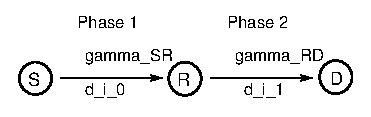
\includegraphics[scale=1.4]{Buffer_Aided_DF_Relaying}
		\caption{Buffer\,-\,aided DF Relaying}
		\label{fig:Buffer_Aided_DF_Relaying}
	\end{figure}
	\item In practice, the nodes in the network have buffers. Thus, we can use the stronger link and wait until the channel conditions of the weaker link have sufficiently improved.
	\item To avoid buffer over\,- or underflow at the relay, we demand that the average rate of the source relay channel (S\,-\,R) is equal to the average rate of the R\,-\,D channel
	\item We introduce a binary selection variable $d(i) $ for time slot $i = \{1,\,2,\,\ldots\} $, where:
	\begin{align*}
		d(i) = 0 \quad &\Rightarrow \quad \text{S transmits, R receives} \\
		d(i) = 1 \quad &\Rightarrow \quad \text{R transmits, D receives}
	\end{align*}
	\item Note: For conventional relaying we have $ d(1) = 0,\, d(2) = 1,\, d(3) = 0,\, d(4) = 1, \ldots $
	\item The average rate in the S\,-\,R link is:
	\begin{align*}
		R_{SR} = \frac{1}{N}\sum_{i=1}^{N}\bigl(1 - d(i)\bigr)\log_2\bigl(1 + \gamma_{SR}(i)\bigr)
	\end{align*}
	and that of the R\,-\,D link is:
	\begin{align*}
		R_{RD} = \frac{1}{N}\sum_{i=1}^{N}d(i)\log_2\bigl(1 + \gamma_{RD}(i)\bigr)
	\end{align*}
	where N denotes the total number of time slots.
	\item $\gamma_{SR}(i) $ and $ \gamma_{RD}(i) $ change from one time slot to the next following e.g. a Rayleigh distribution
	\item At the relay, we have the constraint $ R_{SR} = R_{RD} $ to avoid buffer over\,-\,/\,underflow
	\item To maximize the achievable throughput, we formulate an optimization problem:
	\begin{align*}
		&\underset{d(i) \forall i}{\max}\, R_{RD} \\ 
		\text{subject to:}\, &\text{C1:}\quad R_{RD} = R_{SR} \\
		&\text{C2:}\quad d(i) \in \{0,\,1\}
	\end{align*}
	\item For finite N, this problem is very difficult to solve.
	\item For infinte N, a simple solution exists.
	\item[$\rightarrow$] Solution can be found by Langrange method
	\item Solution $(\text{for }\, N \rightarrow \inf )$: The optimal $d(i) $ is given by:
	\begin{align*}
		d(i) = 
		\begin{cases}
			&1\quad \text{if}\quad \log_2\bigl( 1 + \gamma_{RD}(i)\bigr) \geq \rho \log_2\bigl( 1 + \gamma_{SR}(i)\bigr) \\
			&0\quad \text{otherwise} 
		\end{cases}
\end{align*}	 
	where $\rho $\, is a constant, that only depends on the statistics of $\gamma_{SR}(i) $ and $ \gamma_{RD}(i) $ and can be obtained from (numerical search needed):
	\begin{align*}
		\mathcal{E}_{\gamma_{SR}(i)}\bigl\{\bigl(1 - d(i)\bigr)\log_2\bigl(1 + \gamma_{SR}(i)\bigr)\bigr\} = \mathcal{E}_{\gamma_{RD}(i)}\bigl\{d(i)\cdot\log_2\bigl(1 + \gamma_{RD}(i)\bigr)\bigr\}
	\end{align*}
	\item Since always: the ``best" of two links is selected, this scheme can achieve a diversity gain of $G_d = 2 $ (Rayleigh Fading)
\end{itemize}
\end{document}				